\documentclass[12pt,a4paper]{article}
\usepackage{polski}
\usepackage{wmstitle_lic}
\usepackage{graphicx}
\usepackage{color}
\usepackage{mathtools}
\usepackage{float}
\usepackage{mathrsfs}

\newtheorem{df}{Definicja}[section]
\newtheorem{pr}{Przyk{\l}ad}[section]
\newtheorem{twr}{Twierdzenie}[section]
\newtheorem{pro}{Problem}[section]

\begin{document}

\title{Hipoteza \v Cernego}
\author{Sylwia Klimkiewicz, Adam Jamka}
\promotor{Wit Fory\'s}
\nralbumu{276782, 276765}
\maketitle


%% SEKCJA 1 Podstawowe definicje
\section{Podstawowe definicje.}
%% def 1.1
\begin{df} 
Grafem nazywamy $G=(V,E)$, gdzie $V$ jest niepustym zbiorem, kt\'orego elementy zwane s\k{a} wierzcho{\l}kami a $E$ jest rodzin\k{a} dwuelemntowych podzbior\'ow zbioru $V$, zwanych kraw\k{e}dziami.
$E=\{vw : v,w\in V \}$.
\end{df}
%% def 1.2
\begin{df} 
Niech $G=(V,E)$ b\k{e}dzie grafem. Liczb\k{e} wierzcho{\l}\'ow grafu $G$ nazywamy rz\k{e}dem grafu i oznaczamy $|V|$, natomiast liczb\k{e} kraw\k{e}dzi nazywamy rozmiarem grafu i oznaczamy $|E|$
\end{df}
%% def 1.3
\begin{df} 
Niech $G=(V,E)$ b\k{e}dzie grafem. Zbi\'or s\k{a}siad\'ow wierzcho{\l}ka $v\in V$ $N(v)$ sk{\l}ada si\k{e} z wszystkich wierzcho{\l}k\'ow grafu $G$, takich \.ze istniej\k{a} kraw\k{e}dzie nale\.z\k{a}ce do zbioru $E$, {\l}\k{a}cz\k{a}ce te wierzcho{\l}ki z v. $N(v)=\{w : vw\in E\}$.
\end{df} 
%% def 1.4
\begin{df} 
Niech $G=(V,E)$ b\k{e}dzie grafem. Stopniem wierzcho{\l}ka $v\in V$ nazywamy liczb\k{e} jego s\k{a}siad\'ow i oznaczamy $deg(v)$.
\end{df}
%% def 1.5
\begin{df} 
Graf $G=(V,E)$ jest r-regularny, je\.zeli wszystkie jego wierzcho{\l}ki maj\k{a} stopie\'n r\'owny r.
\end{df} 
%% def 1.6
\begin{df} 
Kraw\k{e}dzi\k{a} skierowan\k{a} lub {\l}ukiem grafu $G=(V,E)$ nazywamy uporz\k{a}dkowan\k{a} par\k{e} wierzcho{\l}k\'ow $e=(v,w)$, gdzie $v\in V$ jest pocz\k{a}tkiem {\l}uku $e$, natomiast $w\in V$ jego ko\'ncem. Graf sk{\l}adaj\k{a}cy si\k{e} z kraw\k{e}dzi skierowanych nazywamy grafem skierowanym.
\end{df}
%% def 1.7
\begin{df} 
Niech $G=(V,E)$ b\k{e}dzie grafem. Ci\k{a}g wierzcho{\l}k\'ow $(v_{1},\ldots,v_{n})$, taki \.ze $\forall_{i}$ $v_{i}\in V$ oraz  $(v_{i-1},v_{i})\in E$ dla $i=2,\ldots,n$ nazywamy \'scie\.zk\k{a} w grafie $G$.
\end{df} 
%% def 1.8
\begin{df} 
Graf $G$ jest sp\'ojny je\'sli dowolne dwa jego wierzcho{\l}ki s\k{a} po{\l}\k{a}czone \'scie\.zk\k{a}.
\end{df}
%% def 1.9
\begin{df} 
Automatem nazywamy tr\'{o}jk\k{e} $\mathscr{A}=(Q, \Sigma, \delta)$, gdzie Q jest zbiorem mo\.{z}liwych stan\'{o}w, $\Sigma$ jest alfabetem, natomiast $\delta:Q x \Sigma \rightarrow$ Q jest funkcj\k{a} definiuj\k{a}c\k{a} 	zachowanie si\k{e} litery nale\.{z}\k{a}cej do alfabetu $\Sigma$ w stanie Q.
\end{df}


%% SEKCJA 2 Wprowadzenie do problemu
\newpage
\section{Wprowadzenie do problemu. Przyk{\l}ady zastosowa\'{n}.}

%%Przykład 2.1
\begin{pr}
\label{pr:przyklad1}
Przyk{\l}adem synchronicznego automatu  $\mathscr{A}$ z czterema stanami Q = \textbraceleft 1, 2, 3, 4\textbraceright  oraz alfabetem sk{\l}adaj\k{a}cym si\k{e} z dw\'{o}ch liter $\Sigma$ = \textbraceleft a, b\textbraceright  mo\.{z}e by\'c poni\.{z}szy graf.
%% Rysunek 1
\begin{figure}[H]
    \centering
    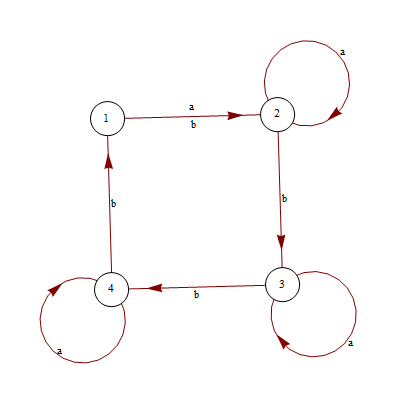
\includegraphics[width=0.62\textwidth]{rysunek1}
    \caption{Synchroniczny automat}
    \label{fig:rysunek1}
\end{figure}

{\L}atwo mo\.{z}emy sprawdzi\'{c}, \.{z}e s{\l}owem resetuj\k{a}cym automat na rysunku \ref{fig:rysunek1} jest \textit{abbbabbba}, co r\'{o}wnowa\.{z}nie mo\.{z}emy zapisa\'{c} \textit{a$b^{3}$a$b^{3}$a}. Pos{\l}ugujac si\k{e} tym s{\l}owem, niezale\.{z}nie od stanu pocz\k{a}tgowego, \'{s}cie\.{z}ka zawsze sko\'{n}czy si\k{e} na wierzcho{\l}ku drugim.\\
\\
\textbf{1}$\xrightarrow{a}$2$\xrightarrow{b}$3$\xrightarrow{b}$4$\xrightarrow{b}$1$\xrightarrow{a}$2$\xrightarrow{b}$3$\xrightarrow{b}$4$\xrightarrow{b}$1$\xrightarrow{a}$\textbf{2}\\
\textbf{2}$\xrightarrow{a}$2$\xrightarrow{b}$3$\xrightarrow{b}$4$\xrightarrow{b}$1$\xrightarrow{a}$2$\xrightarrow{b}$3$\xrightarrow{b}$4$\xrightarrow{b}$1$\xrightarrow{a}$\textbf{2}\\
\textbf{3}$\xrightarrow{a}$3$\xrightarrow{b}$4$\xrightarrow{b}$1$\xrightarrow{b}$2$\xrightarrow{a}$2$\xrightarrow{b}$3$\xrightarrow{b}$4$\xrightarrow{b}$1$\xrightarrow{a}$\textbf{2}\\
\textbf{4}$\xrightarrow{a}$4$\xrightarrow{b}$1$\xrightarrow{b}$2$\xrightarrow{b}$3$\xrightarrow{a}$3$\xrightarrow{b}$4$\xrightarrow{b}$1$\xrightarrow{b}$2$\xrightarrow{a}$\textbf{2}
\end{pr}

Rozwa\.{z}my teraz troszk\k{e} bardziej rozbudowany automat, tak zwany automat Ashby. Przyk{\l}ad ten opisuje jak poradzi\'{c} sobie ze st{\l}umieniem ha{\l}asu generowanego przez dwa \'{z}r\'{o}d{\l}a - \'{s}piew oraz \'{s}miech.

%% Przykład 2.2
\begin{pr}
W tym automacie mamy tyle samo stan\'{o}w co w Przyk{\l}adzie \ref{pr:przyklad1}  Q = \textbraceleft 00, 01, 10, 11\textbraceright, lecz ilo\'{s}\'{c} liter w alfabecie zosta{\l}a zwi\k{e}kszona do czterech $\Sigma$ = \textbraceleft a, b, c, d\textbraceright. Ka\.{z}dy stan sk{\l}ada si\k{e} z dw\'{o}ch cyfr, pierwsza b\k{e}dzie odpowiada{\l}a za ha{\l}as generowany przez \'{s}piew, a druga przez \'{s}miech, gdzie \textit{0} oznacza\'{c} b\k{e}dzie brak ha{\l}asu, natomiast \textit{1} generowanie nieprzyjemnego d\'{z}wi\k{e}ku.

%% Rysunek 2
\begin{figure}[H]
    \centering
    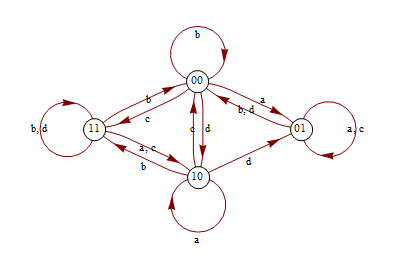
\includegraphics[width=1.05\textwidth]{rysunek2}
    \caption{Automat Ashby}
    \label{fig:rysunek2}
\end{figure}

Rozwa\.{z}aj\k{a}c s{\l}owo \textit{acb} szybko stwierdzimy, \.{z}e jest ono s{\l}owem resetuj\k{a}cym automat przedstawiony na Rysunku \ref{fig:rysunek2}.\\
\\
\textbf{00}$\xrightarrow{a}$01$\xrightarrow{c}$01$\xrightarrow{b}$\textbf{00}\\
\textbf{01}$\xrightarrow{a}$01$\xrightarrow{c}$01$\xrightarrow{b}$\textbf{00}\\
\textbf{10}$\xrightarrow{a}$10$\xrightarrow{c}$00$\xrightarrow{b}$\textbf{00}\\
\textbf{11}$\xrightarrow{a}$01$\xrightarrow{c}$00$\xrightarrow{b}$\textbf{00}\\

Oznacza to, i\.{z} po zastosowaniu tego s{\l}owa ha{\l}as nie b\k{e}dzie generowany ani przez \'{s}piew, ani przez \'{s}miech, a wi\k{e}c b\k{e}dziemy w stanie do kt\'{o}rego d\k{a}\.{z}yli\'{s}my.
\end{pr}

Po przeanalizowaniu powy\.{z}szych przyk{\l}ad\'{o}w dochodzimy do wniosku, i\.{z} po zastosowaniu s{\l}owa resetuj\k{a}cego ko\'{n}czymy prac\k{e} w znanym z g\'{o}ry stanie, lecz nie wiemy z kt\'{o}rego stanu zaczynali\'{s}my.

Nast\k{e}pny przyk{\l}ad poka\.{z}e jakie zastosowanie mo\.{z}e dany problem mie\'{c} w dziedzinie przemys{\l}u, handlu, gdzie np. b\k{e}dziemy pakowa\'{c} jakie\'{s} elementy, kt\'{o}re maj\k{a} okre\'{s}lony kszta{\l}t.

%% Przykład 2.3
\begin{pr}
Przypu\'{s}\'{c}my, \.{z}e nasz przedmiot ma kszta{\l}t wielok\k{a}ta przedstawionego na Rysunku \ref{fig:rysunek3}.

%% Rysunek 3
\begin{figure}[H]
    \centering
    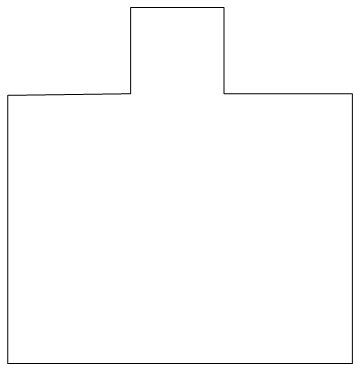
\includegraphics[width=0.23\textwidth]{rysunek3}
    \caption{Wielok\k{a}tny element}
    \label{fig:rysunek3}
\end{figure}


Ka\.{z}dy taki element wk{\l}adamy do pude{\l}ka, lecz zanim to zrobimy musimy je odpowiednio posortowa\'{c}, tak aby mia{\l}y t\k{a} sam\k{a} orientacj\k{e}. Dla u{\l}atwienia przypu\'{s}my, \.{z}e s\k{a} mo\.{z}liwe tylko cztery pozycje tego elementu, kt\'{o}re s\k{a} widoczne na Rysunku \ref{fig:rysunek4}.

%% Rysunek 4
\begin{figure}[H]
    \centering
    
\includegraphics[width=0.87\textwidth]{rysunek4}
    \caption{Mo\.{z}liwe orientacje elementu}
    \label{fig:rysunek4}
\end{figure}

Za{\l}\'{o}\.{z}my, \.{z}e interesuj\k{a}ca dla nas jest druga od lewej strony orientacja elementu. Skorzystamy z lekko zmodyfikowanego automatu, kt\'{o}ry juz wcze\'{s}niej poznali\'{s}my, a dok{\l}adniej z automatu przedstawionego na Rysunku \ref{fig:rysunek1}. G{\l}\'{o}wna zmiana b\k{e}dzie polega{\l}a na tym, i\.{z} mo\.{z}liwe stany, kt\'{o}re automat mo\.{z}e przyj\k{a}\'{c} b\k{e}d\k{a} kolejnymi orientacjami tego elementu.
\\
%% Rysunek 5
\begin{figure}[H]
    \centering
    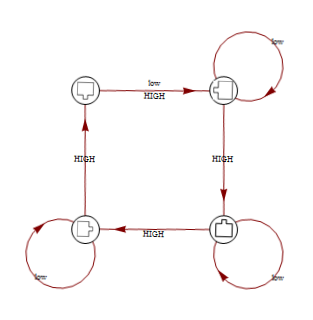
\includegraphics[width=0.7\textwidth]{rysunek5}
    \caption{Zmiana orientacji elementu}
    \label{fig:rysunek5}
\end{figure}

Pami\k{e}taj\k{a}c s{\l}owo resetuj\k{a}ce w automacie z Rysunku \ref{fig:rysunek1} abbbabbba wnioskujemy, \.{z}e s{\l}owem resetuj\k{a}cym automat na Rysunku \ref{fig:rysunek5} jest low-HIGH-HIGH-HIGH-low-HIGH-HIGH-HIGH-low, a stan ko\'{n}cowy to orientacja elementu, kt\'{o}r\k{a} chcieli\'{s}my uzyska\'{c}.
\end{pr}

Jak wida\'{c} nawet dla ma{\l}o skomplikowanego automatu synchronicznego mo\.{z}emy znale\'{z}\'{c} proste, a przede wszystkim z \.{z}ycia wzi\k{e}te zastosowanie, kt\'{o}re oczywi\'{s}cie mo\.{z}emy uog\'{o}lnia\'{c}, a sam automat stara\'{c} si\k{e} rozwija\'{c}, powi\k{e}ksza\'{c}.


%% SEKCJA 3 Algorytm znajdowania słowa sychronizującego
\newpage
\section{Algorytm znajdowania s{\l}owa synchronizuj\k{a}cego.}

Za{\l}\'{o}\.{z}my, \.{z}e mamy dany automat  $\mathscr{A}=(Q, \Sigma, \delta)$. Konstruujemy automat mocy $P(\mathscr{A})$. Jego zbi\'{o}r stan\'{o}w to zbi\'{o}r $P'(Q)$, kt\'{o}ry jest niepustym podzbiorem Q, a funkcja przejscia $\delta$ jest naturalnie rozszerzona do zbioru $P'(Q)x\Sigma$. Inaczej m\'{o}wi\k{a}c dla ka\.{z}dego niepustego podzbioru $P$ zbioru $Q$ oraz $a \epsilon \Sigma$ mamy $\delta(P,a)=\{\delta(p,a) | p\epsilon P\}$.
\\
%% Rysunek 6
\begin{figure}[H]
    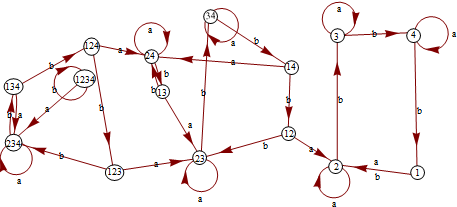
\includegraphics[width=1.1\textwidth]{rysunek6}
    \caption{Automat mocy}
    \label{fig:rysunek6}
\end{figure}

Na Rysunku \ref{fig:rysunek6} przedstawiony zosta{\l} automat mocy dla sko\'{n}czonego automatu przedstawionego na Rysunku \ref{fig:rysunek1}. S{\l}owo $w \epsilon \Sigma$ jest s{\l}owem resetuj\k{a}cym automat $\mathscr{A}$ je\'{s}li w $P(\mathscr{A})$ \'{s}cie\.{z}ka wygenerowana przez to s{\l}owo, zaczynaj\k{a}ca si\k{e} w dowolnym stanie $q \epsilon Q$ ko\'{n}czy si\k{e} zawsze w tym samym wierzcho{\l}ku. W naszym przypadku s{\l}owem resetuj\k{a}cym jest ju\.{z} wcze\'{s}niej znalezione s{\l}owo $ab^3ab^3a$, a wierzcho{\l}kiem ko\'{n}cowym - wierzcho{\l}ek $2$. Ponadto jest to najkr\'{o}tsze s{\l}owo resetuj\k{a}ce. 

Reasumuj\k{a}c algorytm szukania s{\l}owa resetuj\k{a}cego automat $\mathscr{A}$ nie jest skomplikowany. W skr\'{o}cie najpierw tworzymy automat mocy $P(\mathscr{A})$, nast\k{e}pnie szukamy s{\l}owa, dzi\k{e}ki kt\'{o}remu startuj\k{a}c z dowolnego stanu dostaniemy si\k{e} do jednego, tego samego wierzcho{\l}ka - mo\.{z}emy tutaj zastosowa\'{c} algorytm przeszukiwania 
wszerz (BFS), kt\'{o}ry pomo\.{z}e znale\'{z}\'{c} takie s{\l}owo albo stwierdzi\'{c}, i\.{z} ono nie istenieje. Problem jednak w tym, \.{z}e rozmiar automatu mocy $P(\mathscr{A})$ jest wyk{\l}adniczo wi\k{e}kszy od rozmiaru automatu $\mathscr{A}$. Otrzymany w ten spos\'{o}b algorytm ma z{\l}o\.{z}ono\'{s}\'{c} wielomianow\k{a}.


%% SEKCJA 4 WKW na to, żeby graf był synchronizowalny z dowodem
\newpage
\section{Warunek konieczny i wystarczaj\k{a}cy na synchronizowalno\'{s}\'{c} automatu.}

Oczywistym faktem jest, \.{z}e nie ka\.{z}dy sko\'{n}czony automat jest synchroniczny. Nasuwa si\k{e} wi\k{e}c pytanie, je\'{s}li mamy dany sko\'{n}czony automat $\mathscr{A}=(Q, \Sigma, \delta)$, jak stwierdzi\'{c} czy jest on synchroniczny czy nie?

%% Twierdzenie 3.1
\begin{twr}
\label{tw:twierdzenie1}
Sko\'{n}czony automat $\mathscr{A}=(Q, \Sigma, \delta)$ jest synchroniczny wtedy i tylko wtedy, gdy dla ka\.{z}dego stanu $q, q' \epsilon Q$ istnieje s{\l}owo $w \epsilon \Sigma$ takie, \.{z}e $\delta(q,w)=\delta(q',w)$.
\end{twr}

Zredukujmy problem z Twierdzenia \ref{tw:twierdzenie1} dotycz\k{a}cego synchronizowalno\'{s}ci automatu do problemu zasi\k{e}gu w podautomacie $P^{[2]}(\mathscr{A})$ automatu mocy $P(\mathscr{A})$, kt\'{o}rego zbi\'{o}r stan\'{o}w jest z{\l}o\.{z}ony z jednoelementowych oraz dwuelementowych podzbior\'{o}w zbioru $Q$. Podautomat posiada $\frac{|Q|(|Q|+1)}{2}$ stan\'{o}w. Algorytm BFS, czyli przeszukiwanie grafu wszerz, rozwi\k{a}zuje ten problem w czasie $O(|Q|^2*|\Sigma|)$. To ograniczenie pozwala wnioskowa\'{c}, i\.{z} je\'{s}li s{\l}owo resetuj\k{a}ce nie istnieje dostaniemy o tym stosown\k{a} informacj\k{e} w sko\'{n}czonej jednostce czasu, kt\'{o}rej wielko\'{s}\'{c} zale\.{z}y od rozmiaru zbioru stan\'{o}w oraz alfabetu. Je\'{s}li natomiast automat $\mathscr{A}$ jest synchroniczny, jako wynik algorytmu wyprodukowane zostanie s{\l}owo resetuj\k{a}ce ten automat. Najlepszy znany algorytm, kt\'{o}ry jako wynik daje s{\l}owo resetuj\k{a}ce posiada z{\l}o\.{z}ono\'{s}\'{c} czasow\k{a} rz\k{e}du $O(|Q|^3+|Q|^2*|\Sigma|)$ oraz z{\l}o\.{z}ono\'{s}\'{c} pami\k{e}ciow\k{a} rz\k{e}du $O(|Q|^2*|\Sigma|)$, nie licz\k{a}c pami\k{e}ci potrzebnej na zapisanie wyniku, kt\'{o}ra jest rz\k{e}du $O(|Q|^3)$.


%% SEKCJA 5 Problem długości słowa synchronizującego
\newpage
\section{Problem d{\l}ugo\'{s}ci s{\l}owa synchronizuj\k{a}cego.}

Automat mocy synchronicznego automatu mo\.ze by\'c u\.zyteczny w konstruowaniu najkr\'otszych s{\l}\'ow resetuj\k{a}cych, co jest zwi\k{a}zane z najkr\'otsz\k{a} \'scie\.zk\k{a} w automacie mocy od ca{\l}ego zestawu stan\'ow, a\.z do singletona. Oczywi\'scie w najgorszym przypadku wymaga to wyk{\l}adniczgo czasu. Niemniej jednak by{\l}y pr\'oby zaimplemetowania tego podej\'scia. Mo\.zna mie\'c nadziej\k{e}, \.ze odpowiednie obliczenia dla "wielomianowego" subautomatu $P^{[2]}(\mathscr{A})$ pozwol\k{a} uzyska\'c algorytm wielomianowy. Jednak, ma{\l}o prawdopodobne jest to, \.ze istnieje jakikolwiek rozs\k{a}dny algorytm znajdowania najkr\'otszego s{\l}owa resetuj\k{a}cego w przypadku og\'olnym.\\ 
\\
Rozwa\.zmy teraz dwa nast\k{e}puj\k{a}ce problemy:

%% Problem 4.1
\begin{pro}
(Kr\'otkie s{\l}owo resetuj\k{a}ce.) Maj\k{a}c automat synchroniczny  $\mathscr{A}=(Q, \Sigma, \delta)$ i liczb\k{e} naturaln\k{a} $l$, czy prawd\k{a} jest to, \.ze $\mathscr{A}$ posiada s{\l}owo resetuj\k{a}ce o d{\l}ugo\'sci $l$?
\end{pro}

%% Problem 4.2
\begin{pro} (Najkr\'otsze s{\l}owo resetuj\k{a}ce.) Maj\k{a}c automat synchroniczny  $\mathscr{A}=(Q, \Sigma, \delta)$ i liczb\k{e} naturaln\k{a} $l$, czy prawd\k{a} jest to, \.ze minimalna  d{\l}ugo\'s\'c s{\l}owa resetuj\k{a}cego automat $\mathscr{A}$ jesr r\'owna $l$?
\end{pro}

Oczywi\'scie problem 3.1 nale\.zy do klasy z{\l}o\.zono\'sci NP; mo\.zna nie -deterministycznie odgadn\k{a}\'c s{\l}owo $w\in\Sigma^{*}$ o d{\l}ugo\'sci $l$, a nast\k{e}pnie sprawdzi\'c czy $w$ jest s{\l}owem resetuj\k{a}cym automat $\mathscr{A}$ w czasie wielomianowym. David Eppstein udowodni{\l}, w 1990 roku \.ze problem 3.1 jest NP-trudny przez wielomianow\k{a} redukcj\k{e} z problemu NP-zupe{\l}nego. Dlatego problem 3.1 jest NP-zupe{\l}ny. Z dowodu tego {\l}atwo wynika, \.ze problem 3.2 jest NP-trudny. Wojciech Samotij pokaza{\l}, \.ze negacja NP-zupe{\l}no\'sci mo\.ze by\'c wielomianowo zredukowana do problemu 3.2, sk\k{a}d ostatni problem r\'ownie\.z jest coNP-trudny. Jako konsekwencja problem 3.2 nie mo\.ze nale\.ze\'c do klasy NP je\.zeli nieprawd\k{a} jest, \.ze NP=coNP, co jest powszechnie uwa\.zane za ma{\l}o prawdopodobne. Innymi s{\l}owy, nawet nie-deterministyczny algorytm nie mo\.ze znale\'z\'c minimalnej d{\l}ugo\'sci s{\l}owa resetuj\k{a}cego dla danego automatu synchronicznego w czasie wielomianowym.

Z drugiej strony wyczerpuj\k{a}ce przeszukiwanie wszysztkich s{\l}\'ow nad alfabetem $\Sigma$ o d{\l}ugo\'sci $\leq l$ mo\.ze zosta\'c wykonane w pami\k{e}ci wielomianowej, a w rzeczywisto\'sci w liniowej. Dlatego problem 3.2 nale\.zy do klasy z{\l}o\.zono\'sci PSPACE. Pytanie o precyzyjne ulokowanie tego problemu w odniesieniu do hierarchii wielomian\'ow wci\k{a}\.z pozostaje otwarte. 

Trudno\'s\'c problemu decyzyjnego w 3.1 implikuje to, \.ze jego zoptymalizowana wersja, w kt\'orej szuka si\k{e} s{\l}owa resetuj\k{a}cego o minimalnej d{l}ugo\'sci dla danego automatu synchronicznego r\'ownie\.z jest trudna. Jednak\.ze to nie wyklucza tego, \.ze problem optymalizacji mo\.ze dopuszcza\.c wielomianowy algorytm aproksymacji, co wi\k{e}cej wszystkie istniej\k{a}ce dowody tego, \.ze problem 3.1 jest NP-trudny s\k{a} zgodne z  przypuszczeniem \.ze taki algorytm istnieje. Orzeczenie czy to przypuszczenie jest prawdziwe, czy te\.z nie stanowi ciekawy problem badawczy. Carl Pixley w 1992 zasugewowa{\l} heurystyczny algorytm znajdowania kr\'otkiego s{\l}owa resetuj\k{a}cego dla automatu synchronicznego, kt\'ory zosta{\l} wykorzystany do wykonywania zadowalaj\k{a}cych ilo\'sci test\'ow. P\'o\'zniej algorytmy szukaj\k{a}ce kr\'otkich s{\l}\'ow resetuj\k{a}cych zosta{\l}y zaimplementowane przez Avrahama Trahtmana.


%% SEKCJA 6 Hipoteza Cernego
\newpage
\section{Hipoteza \v Cernego.}

W tym rozdziale om\'{o}wimy otwarty do tej pory problem i wyniki, zwi\k{a}zane z nast\k{e}puj\k{a}cym pytaniem: posiadaj\k{a}c zadane $n \in N$ jak d{\l}ugie mo\.ze by\'c s{\l}owo resetuj\k{a}ce sko\'nczony automat synchroniczny o $n$ stanach? 

Przywo{\l}ajmy najpierw konstrukcj\k{e} \v Cernego. Dla liczby naturalnej $n>1$ oznaczmy $C_{n}$ jako sko\'nczony automat synchroniczny, kt\'orego stany s\k{a} resztami modulo $n$, a litery wej\'sciowe $a$ i $b$ dzia{\l}aj\k{a} nast\k{e}puj\k{a}co:\\
\\
$\delta(0,a)=1$\\
$\delta(m,a)=m$ for $0<m<n$\\
$\delta(m,b)=m+1(modn)$
%% Rysunek 
\begin{figure}[H]
    \centering
    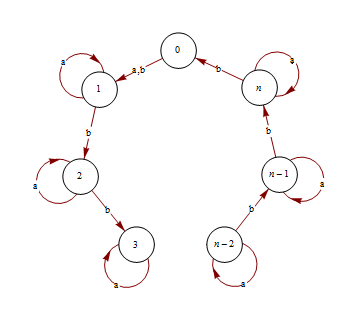
\includegraphics[width=0.8\textwidth]{rysunek7}
    \caption{Automat $C_{n}$}
    \label{fig:rysunek7}
\end{figure}

\v Cerny udowodni{\l}, \.ze $C_{n}$ jest automatem synchronicznym i najkr\'otszym resetuj\k{a}cym go s{\l}owem jest $(ab^{n-1})^{n-2}a$ o d{\l}ugo\'sci $(n-1)^{2}$. Zatem je\'sli zdefiniujemy funkcj\k{e} \v Cernego $C(n)$ jako maksimum d{\l}ugo\'sci najkr\'otszego s{\l}owa resetuj\k{a}cego automat synchroniczny posiadaj\k{a}cy $n$ stan\'ow powy\.zsza w{\l}asno\'s\'c dla ci\k{a}gu $\{C_{n}\}_{n=2,3,\ldots}$ daje nier\'owno\'s\'c: $C(n)\leq(n-1)^{2}$. Hipoteza \v Cernego m\'owi \.ze tak naprawd\k{e} zachodzi r\'owno\'s\'c: $C(n)=(n-1)^{2}$. W literaturze mo\.zna spotka\'c nawi\k{a}zania do tego,\.ze praca \v Cernego z 1964 roku jest \'zr\'od{\l}em tej hipotezy, ale tak naprawd\k{e} nie zosta{\l}a ona wtedy sformu{\l}owana. Jedkak\.ze \v Cerny zaobserwowa{\l}, \.ze: $(n-1)^{2}\leq C(n)\leq2^{n}-n-1$ i za{\l}\k{a}czy{\l} do tego nast\k{e}puj\k{a}c\k{a} uwag\k{e}: "R\'o\.znica pomi\k{e}dzy granicami wzrasta szybko i nale\.zy je zacie\'sni\'c. Mo\.zna si\k{e} spodziewa\'c polepszenia g{\l}\'ownie dla g\'ornej granicy."

Hipoteza w swej obecnej postaci zosta{\l}a sformu{\l}owana troch\k{e} p\'ozniej, po tym jak oczekiwania zawarte w powy\.zszym cytacie zosta{\l}y potwierdzone przez Peter'a Starke'a, kt\'ory pomniejszy{\l} g\'orn\k{a} granic\k{e} do $1+\frac{n(n-1)(n-2)}{2}$, co by{\l}o pierwsz\k{a} wielomianow\k{a} g\'orn\k{a} granic\k{a} dla $C(n)$. \v Cerny wypowiedzia{\l} hipotez\k{e} $C(n)=(n-1)^{2}$ na Konferencji Cybernetycznej  w Bratys{\l}awie w 1969 roku, natomiast w druku hipoteza pojawi{\l}a si\k{e} po raz pierwszy w 1971 roku.


%% SEKCJA 7 Oszacowanie długości słowa synchronizującego z dowodem
\newpage
\section{Oszacowanie d{\l}ugo\'{s}ci s{\l}owa synchronizuj\k{a}cego.}

W rozdziale sz\'ostym przedstawiona zosta{\l}a tre\'s\'c hipotezy \v Cernego oraz pewne g\'orne oszacowania funkcji $C_{n}$, kt\'ore z  biegiem czasu stawa{\l}y si\k{e} coraz dok{\l}adniejsze. Najdok{\l}adniejsze znane g\'orne ograniczenie funkcji \v Cernego gwarantuje to, \.ze dla ka\.zdego automatu synchronicznego posiadaj\k{a}cego $n$ stan\'ow istnieje s{\l}owo resetuj\k{a}ce o d{\l}ugo\'sci $\frac{n^{3}-n}{6}$.

\end{document}


\begin{comment}
PYTANIA

Często używam BFS-a, może po krótce gdzieś go opisać? Jakiś jeden krótki przykład?

Sekcja 3:
Może jakieś inne opracowanie tego dowodu? Co to jest P^[2](A)? Czy to na pewno jest podautomat automatu mocy P(A)? Czy dobrze został przetłumaczony fragment "reachability problem" na problem zasięgu w podautomacie P^[2](A)? Algorytm BFS daje tylko informację o tym czy słowo synchronizujące istnieje, a żeby znaleźć to słowo trzeba użyć tego algorytmu o złożoności O(|Q|^3+|Q|^2*|\Sigma|)?

\end{comment}
